\documentclass[12pt]{amsart}
% packages
\usepackage{graphicx}
\usepackage{setspace}
\usepackage{amssymb,amsmath,amsthm,amsfonts,amscd}
\usepackage{hyperref}
\usepackage{color}
\usepackage{booktabs}
\usepackage{tabularx}
\usepackage{enumitem}
\usepackage[retainorgcmds]{IEEEtrantools}
\usepackage[notref,notcite,final]{showkeys}
\usepackage[final]{pdfpages}
\usepackage{fancyhdr}
\usepackage{upgreek}
\usepackage{multicol}
\usepackage{fontawesome}
\usepackage{halloweenmath}
% set margin as 0.75in
\usepackage[margin=0.75in]{geometry}

% tikz-related settings
\usepackage{tkz-berge}
\usetikzlibrary{calc,quotes}
\usetikzlibrary{arrows.meta}
\usetikzlibrary{positioning, automata}
\usetikzlibrary{decorations.pathreplacing}

%% For table
\usepackage{tikz}
\usetikzlibrary{tikzmark}

% theorem environments with italic font
\newtheorem{thm}{Theorem}[section]
\newtheorem*{thm*}{Theorem}
\newtheorem{lemma}[thm]{Lemma}
\newtheorem{prop}[thm]{Proposition}
\newtheorem{claim}[thm]{Claim}
\newtheorem{corollary}[thm]{Corollary}
\newtheorem{conjecture}[thm]{Conjecture}
\newtheorem{question}[thm]{Question}
\newtheorem{procedure}[thm]{Procedure}
\newtheorem{assumption}[thm]{Assumption}

% theorem environments with roman font (use lower-case version in body
% of text, e.g., \begin{example} rather than \begin{Example})
\newtheorem{Definition}[thm]{Definition}
\newenvironment{definition}
{\begin{Definition}\rm}{\end{Definition}}
\newtheorem{Example}[thm]{Example}
\newenvironment{example}
{\begin{Example}\rm}{\end{Example}}

\theoremstyle{definition}
\newtheorem{remark}[thm]{\textbf{Remark}}

% special sets
\newcommand{\A}{\mathbb{A}}
\newcommand{\C}{\mathbb{C}}
\newcommand{\F}{\mathbb{F}}
\newcommand{\N}{\mathbb{N}}
\newcommand{\Q}{\mathbb{Q}}
\newcommand{\R}{\mathbb{R}}
\newcommand{\Z}{\mathbb{Z}}
\newcommand{\cals}{\mathcal{S}}
\newcommand{\ZZ}{\mathbb{Z}_{\ge 0}}
\newcommand{\cala}{\mathcal{A}}
\newcommand{\calb}{\mathcal{B}}
\newcommand{\cald}{\mathcal{D}}
\newcommand{\calh}{\mathcal{H}}
\newcommand{\call}{\mathcal{L}}
\newcommand{\calr}{\mathcal{R}}
\newcommand{\la}{\mathbf{a}}
\newcommand{\lgl}{\mathfrak{gl}}
\newcommand{\lsl}{\mathfrak{sl}}
\newcommand{\lieg}{\mathfrak{g}}

% math operators
\DeclareMathOperator{\kernel}{\mathrm{ker}}
\DeclareMathOperator{\image}{\mathrm{im}}
\DeclareMathOperator{\rad}{\mathrm{rad}}
\DeclareMathOperator{\id}{\mathrm{id}}
\DeclareMathOperator{\hum}{[\mathrm{Hum}]}
\DeclareMathOperator{\eh}{[\mathrm{EH}]}
\DeclareMathOperator{\lcm}{\mathrm{lcm}}
\DeclareMathOperator{\Aut}{\mathrm{Aut}}
\DeclareMathOperator{\Inn}{\mathrm{Inn}}
\DeclareMathOperator{\Out}{\mathrm{Out}}
\DeclareMathOperator{\Gal}{\mathrm{Gal}}


% frequently used shorthands
\newcommand{\ra}{\rightarrow}
\newcommand{\se}{\subseteq}
\newcommand{\ip}[1]{\langle#1\rangle}
\newcommand{\dual}{^*}
\newcommand{\inverse}{^{-1}}
\newcommand{\norm}[2]{\|#1\|_{#2}}
\newcommand{\abs}[1]{\lvert #1 \rvert}
\newcommand{\Abs}[1]{\bigg| #1 \bigg|}
\newcommand\bm[1]{\begin{bmatrix}#1\end{bmatrix}}
\newcommand{\op}{\text{op}}

% nicer looking empty set
\let\oldemptyset\emptyset
\let\emptyset\varnothing

\setlist[enumerate,1]{topsep=1em,leftmargin=1.8em, itemsep=0.5em, label=\textup{(}\arabic*\textup{)}}
\setlist[enumerate,2]{topsep=0.5em,leftmargin=3em, itemsep=0.3em}

%pagestyle
%\pagestyle{fancy} 

\begin{document}
\begin{center}
    \textsc{Math 501. HW $C_3+4$\\ Ian Jorquera\\ Collaborators: people in the people places}
\end{center}
\vspace{1em}
% See http://www.mathematicalgemstones.com/maria/Math501Fall22.php
% for problems

% sage: https://sagecell.sagemath.org/
\begin{itemize}[align=left]
\item[\textbf{Problem $C_2$ part a}] %(1+) (2 points)
    \;\\\\
    Consider the graph $G=(V,E)$ where $V=\{0,\dots,d-1\}^{n-1}$, the sequences of length $n-1$. And an edge exists between the sequences $(c_1c_2\dots c_{n-1})$ and $(\hat{c}_1\hat{c}_2\dots \hat{c}_{n-1})$ if the subsequences $(c_2c_3\dots c_{n-1})$ and $(\hat{c}_1\hat{c}_2\dots \hat{c}_{n-2})$ are the same. An edge corresponds to the string of length $n$ that is $c_1c_2\dots c_{n-1}\hat{c}_{n-1}$, and we will denote each edge as this string. First we will show that this graph is connected. Consider two vertices or sequences $(c_1c_2\dots c_{n-1})$ and $(\hat{c}_1\hat{c}_2\dots \hat{c}_{n-1})$. And notice that there exists the path $(c_1c_2\dots c_{n-1})\ra (c_2\dots c_{n-1}\hat{c}_1)\ra (c_3\dots c_{n-1}\hat{c}_1\hat{c}_2)\ra\dots\ra ({c}_{n-1}\hat{c}_1\hat{c}_2\dots \hat{c}_{n-2})\ra (\hat{c}_1\hat{c}_2\dots \hat{c}_{n-1})$. So $G$ is connected. Furthermore we will also show that $G$ is balanced. Consider a vertex $(c_1c_2\dots c_{n-1})$ and consider the out going edges. These are the edges going to vertices of the form $(c_2\dots c_{n-1}\hat{c})$ where $\hat{c}\in\{0,\dots,d-1\}$ of which there are $d$ such edges. The incoming edges are the edges coming from vertices of the form $(\hat{c}c_1c_2\dots c_{n-2})$ where $\hat{c}\in\{0,\dots,d-1\}$ of which there are $d$ such edges. So the in degree and out degree of any vertex is $d$, and so the graph is balanced. This means there will be a Eulerian tour. Because there are $d^{n-1}$ vertices with $d$ outgoing edges for each vertex there are $2^n$ edges, meaning a Eulerian tour will contain all strings of length $n$. To see this more clearly notice that any such string $(c_1c_2\dots c_{n})$ is the edge between $(c_1c_2\dots c_{n-1}$ and $(c_2c_3\dots c_{n}$. Now from a Eulerian tour in the graph we can construct a d-ary de Bruijn sequence: for any starting vertex $(c_1c_2\dots c_{n-1})$ in the tour the d-ary de Bruijn sequence will start with the sequence from the starting vertex. Then for all but the last $n-1$ vertices in the tour we will include the last character in the sequence of each vertex. Notice that because a d-ary de Bruijn sequence is circular the last $n-1$ vertieces in the tour will be sequences overalpping with the characters from the first vertex. This means the constructed subsequences is of length $n-1+2^{d}-(n+1)=2^d$. And a d-ary de Bruijn sequence will always exist.\\
    
\item[\textbf{Problem $|\mathcal{T}(\{\mathwitch, \bigpumpkin, \mathbat\})|$}] %(2-) (3 points)
    \;\\\\
    Ian's loopdeedoo Theorem: Let $G=(V,E)$ be an undirected graph. Then $G$ has an undirected Eulerian tour if and only if $G=(V,E)$ is connected and the degree(not including loops) of every $u\in V$ is even. \\

    Proof: Let $G=(V,E)$ be a undirected graph that contains an undirected Eulerian tour starting and ended at $v_i\in V$. And consider any two vertices $u,v\in V$ and notice that because $u$ and $v$ lie on the tour, there must be a walk between them, along the tour, and so $G$ must be connected. Now consider any vertex $v\in V$, and because the tour uses every edge exactly once, we know that it travels to $v$ as often as it leave $v$. This follows from the fact that for $v\neq v_i$, when the tour travels through $v$ it will travel along two edges incident on $v$, the edge it enters and the edge it leaves. For $v_i$ the same is true as a vertex along the tour, and because the tour starts and ends at $v_i$ the edges it starts and ends at are also incident on $v_i$. And so $G$ must be connected and each vertex has even degree .\\

    Now let $G=(V,E)$ be a undirected graph that is connected and the degree(not including loops) of every $u\in V$ is even. And consider a walk of maximal length with no repeated edges $(v_1,e_1,v_2,e_2,\dots,e_{n-1}v_n)$. If $v_1\neq v_n$ then the walk would enter $v_n$ one more time then it leaves, this means that the walk would have only utilized an odd number of the edges incident on $v_n$, and because $G$ has vertices with even degree we would be able to extend the walk by one edge. This means a maximal walk in $G$ without repeated edges would be a tour $(v_1,e_1,v_2,e_2,\dots,e_{n-1}v_1)$. Now assume that there is an edge $e\in E$ that is indecent on $v_i\in V$ that is not used in the maximal walk. Because $G$ is connected we can assume that $v_i$ is in the maximal walk. If it was not there would have to exist a vertex $v'_i$ with an edge $e'$ incident on $v'_i$ not in the maximal walk that would be contained in a walk between $v_i$ and $v'_i$. Now notice that if this is the case, an unused edge exists incident to the vertex $v_i$ on the maximal walk where $e$ is between $v_i$ and $v'$. This means we can create the walk $(v_i, e_i\dots,e_{n-1}v_1,e_1,v_2,e_2,\dots, e_{i-1}, v_i,e,v')$ which is strictly bigger. Meaning any maximal walk must contain all edges and must start and end at a single vertex. This means a Eulerian tour exists.\\

    \item[\textbf{Problem $R(4,4)-14$}] %(2-) (3 points)
    \iffalse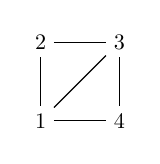
\begin{tikzpicture}
    
    % Add or remove nodes here, use the tuple for location
    \begin{scope}[every node/.style={scale=.8}]
    \node (A) at (0,0) {1};
    \node (B) at (0,10mm) {2};
    \node (C) at (10mm,10mm) {3};
    \node (D) at (10mm,0) {4};
    \end{scope}

    % forward(red)
    % Remove or add new edges here
    \begin{scope}[>={Stealth[black]},
              every edge/.style={draw=black, thin}]. % you can change the color of the edges here
    \path [-] (A) edge (B);
    \path [-] (B) edge (C);
    \path [-] (C) edge (D);
    \path [-] (A) edge (D);
    \path [-] (A) edge (C);
    \end{scope}

    \end{tikzpicture}
    \fi
    \;\\
    \begin{itemize}
        \item[(a)] % 1+ (2 points)
        We will prove this using induction. Notice first that $A^1=A$ is the matrix whose $i,j$ entry are the walks of length $1$ between $i$ and $j$, which is exactly the number of edges between $i$ and $j$ or $a_{ij}$. Now fix $n>1$ and consider the matrix product $A^n=A^{n-1}A$. Where the product of these matrices is $(A^n)_{ij}=\sum_{k=1}^{n}(A^{n-1})_{ik}\cdot a_{kj}$. Where by the inductive hypothesis $(A^{n-1})_{ik}$ counts the number of walks from $i$ to $k$ of length exactly $n-1$, and so $(A^{n-1})_{ik}\cdot a_{kj}$ counts the walks of length $n$ from $i$ to $j$ whose second to last vertex was at $k$. This means that by summing over all $k$ we are counting all walks of length $n$. So $(A^n)_{ij}=\sum_{k=1}^{n}(A^{n-1})_{ik}a_{kj}$ counts the number of walks from $i$ to $j$ of length exactly $n$.\\
        
        \item[(d)] % 2- (3 points)
         Let $b_n$ represent the number of sequences of length $n+1$ that start with a $1$ and end with an $3$ such that there are no $22$ or $23$ subsequences. We can represent these sequences as the sequences of visited vertices on the walks of a graph that start at $1$ and end at $3$ where $(2,2)$ and $(2,3)$ are not edges. That is we have the following graph $G=(V,E)$ where $V=[3]$ and $E=\{(1,1),(1,2),(1,3),(2,1),(3,1),(3,2),(3,3)\}$ which looks like

        \begin{center}
            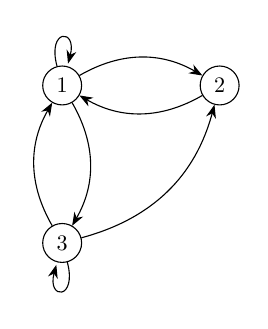
\begin{tikzpicture}
    
        % Add or remove nodes here, use the tuple for location
        \begin{scope}[every node/.style={circle,draw,scale=.8}]
        \node (A) at (0,2) {1};
        \node (B) at (2,2) {2};
        \node (C) at (0,0) {3};
        \end{scope}
    
        % forward(red)
        % Remove or add new edges here
        \begin{scope}[>={Stealth[black]},
                  every edge/.style={draw=black, thin}]. % you can change the color of the edges here
        \path [->] (A) edge[loop above] (A);
        \path [->] (A) edge[bend left, above] (B);
        \path [->] (A) edge[bend left, above] (C);
        \path [->] (B) edge[bend left, above] (A);
        \path [->] (C) edge[bend left, above] (A);
        \path [->] (C) edge[bend right, above] (B);
        \path [->] (C) edge[loop below] (B);
        \end{scope}
    
        \end{tikzpicture}
        \end{center}

        And whose adjacency Matrix is 
        $$A=\begin{pmatrix}
            1 & 1 & 1\\ 1 & 0 & 0\\ 1 & 1 & 1\\
        \end{pmatrix}$$
        With the graph above we have that $b_n$ counts the number of walks on $G$ of length $n$ that start at $1$ and end at $3$. %prove bijection?
        From part c we know that 
        $\sum_{n=0}^{\infty}b_nx^n=\frac{\det(I_3-Ax;3,1)}{\det(I_3-Ax)}=\frac{x}{1-2x-x^2}$. $1-2x-x^2=(1-r_1x)(1-r_2x)$ where $r_1$ and $r_2$ are $1\pm \sqrt{2}$. Which means that $b_n=a(1+ \sqrt{2})^n+b(1- \sqrt{2})^n$. Furthermore we know that $b_0=a+b=0$ meaning $b=-a$ and $b_1=a(1+ \sqrt{2})+b(1- \sqrt{2})=a(1+ \sqrt{2})-a(1- \sqrt{2})=2$. This means that $a=\frac{\sqrt 2}{4}$ and $b=-\frac{\sqrt 2}{4}$. And so we have that $b_n=\frac{\sqrt 2}{4}(1+ \sqrt{2})^n-\frac{\sqrt 2}{4}(1- \sqrt{2})^n$
    \end{itemize}

    
\end{itemize}

\end{document}


